%======================================================================
In this chapter we describe our experimental setup and procedures, as well as the results we obtained when studing the absorbance of semiconducting CNTs.
\section{Bandgap Overlap}
Table shows all hollow-core fiber types available from ThorLabs and the central operating wavelengths for air-filled and D${}_2$O-filled fibers.
The “air” range can be used for fibers that are selectively core-filled with D${}_2$O.
The ranges for HC1550 and HC800B are approximated from spectrum measurements and HC2000 and HC1060 are taken from ThorLabs datasheets.
The D${}_2$O central wavelengths are calculated using the band-gap shift equation.

\begin{tabularx}{0.8\textwidth} { 
		| >{\centering\arraybackslash}X 
		| >{\centering\arraybackslash}X 
		| >{\centering\arraybackslash}X 
		| >{\centering\arraybackslash}X | }
	\hline
	HCPCF & $\lambda_{AIR}$ (nm) & $\lambda_{D_2O}$(nm) & Range (nm)\\
	\hline
	HC2000 & 2000 & 1144 & 250\\
	\hline
	HC1550 & 1550 & 887 & 500\\
	\hline
	HC1060 & 1060 & 606& 100\\
	\hline
	HC800B & 800 & 457 & 200\\
	\hline	
\end{tabularx}
\captionof{table}{ Thorlabs fiber bandgap shift. \label{bgoverlap}}

\begin{figure}[h]
	\centering
	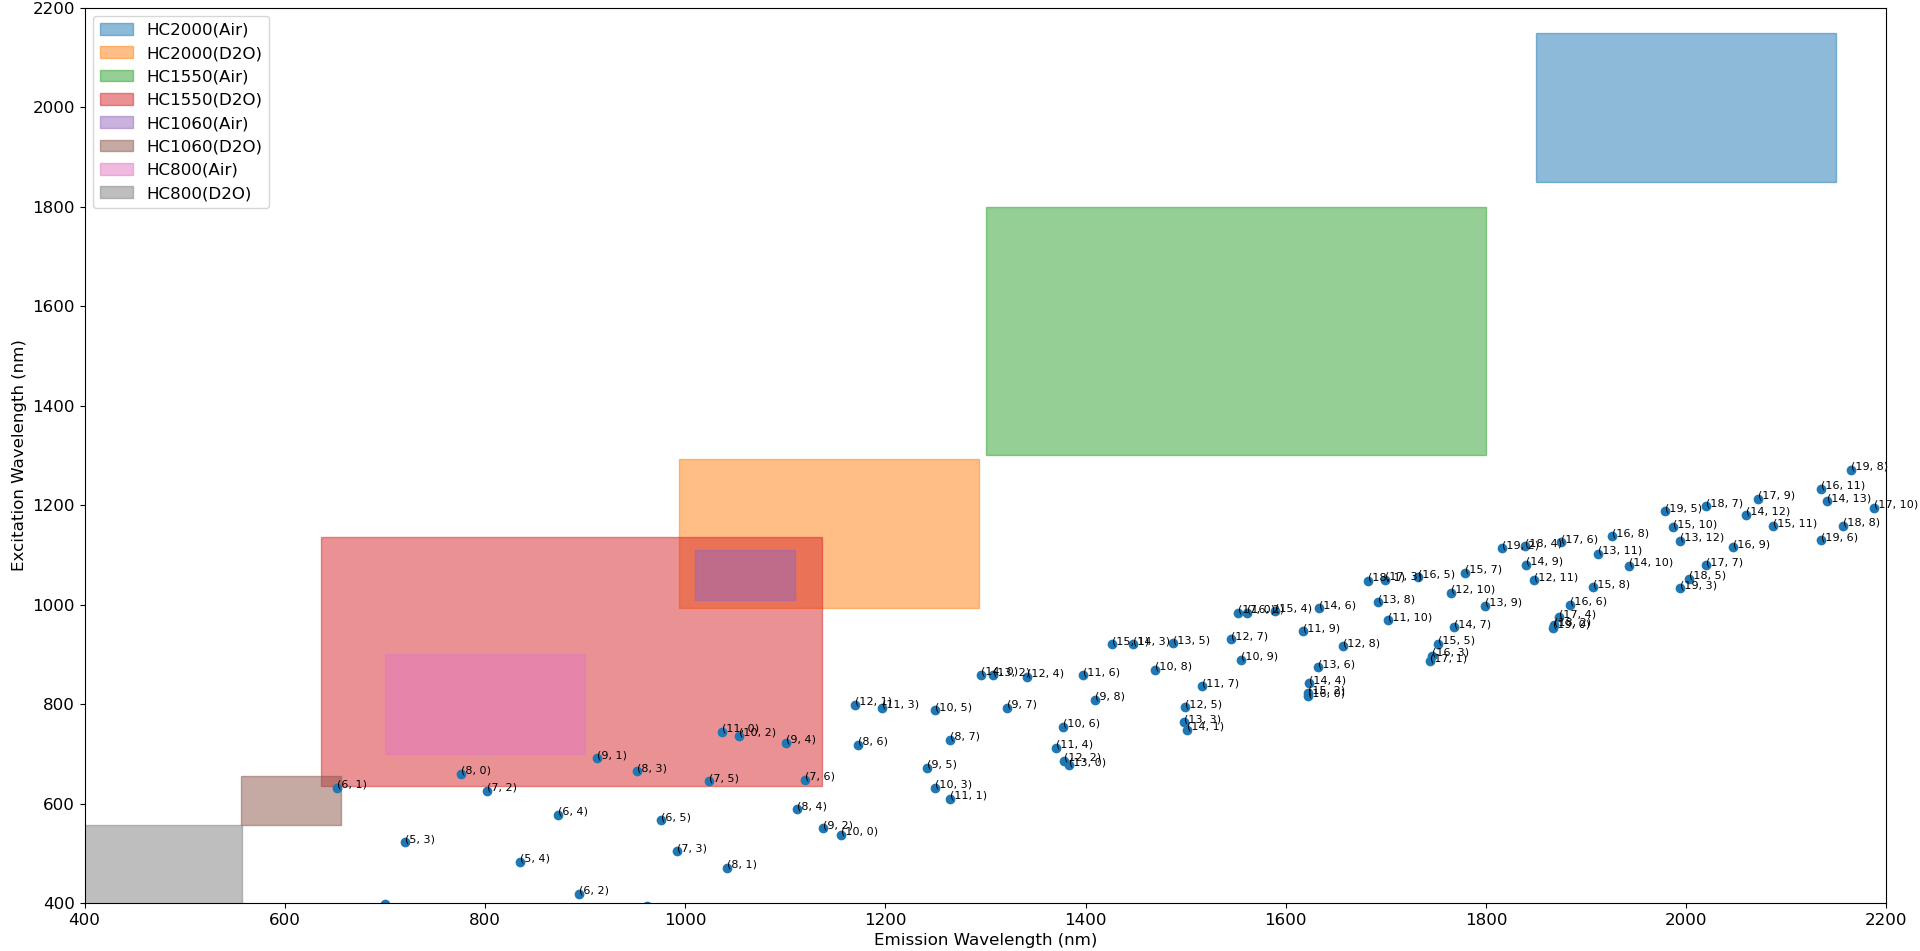
\includegraphics[width=\textwidth]{./Figures/CNTs/fibers_cnt.png}
	\caption{ Hollow-core fiber bandgap overlayed on CNT emission vs. excitation wavelengths }
	\label{fig:cntoverlap}
\end{figure}

\begin{figure}[h]
	
	\begin{minipage}{0.55\linewidth}
		\begin{tabularx}{\linewidth} { 
				| >{\centering\arraybackslash}X 
				| >{\centering\arraybackslash}X 
				| >{\centering\arraybackslash}X 
				| >{\centering\arraybackslash}X 
				| >{\centering\arraybackslash}X
				| >{\centering\arraybackslash}X
				| >{\centering\arraybackslash}X | }
			\hline
			$(n,m)$ & $dt$ (nm)	& $\Theta$ (deg) & 	$\lambda_{11}$ (nm)	 & $\lambda_{22}$ (nm)\\
			\hline
			(6, 1) & 0.52 & 0.13 & 652.62 & 631.79\\
			\hline
			(7, 2) & 0.65 & 0.21 & 802.05 & 625.92\\
			\hline
			(7, 5) & 0.83 & 0.43 & 1023.74 & 645.33\\
			\hline
			(7, 6)  & 0.89 & 27.46 & 1119.76 & 647.64\\
			\hline
			(8, 0) & 0.64 & 0 & 776.01 & 660.25\\
			\hline
			(8, 3) & 0.78 & 0.27 & 951.61 & 665.39\\
			\hline
			(9, 1) & 0.76 & 0.09 & 912.1 & 691.29\\
			\hline
			(9, 4)  & 0.92 & 0.31 & 1100.63 & 722.39\\
			\hline
			(10, 2) & 0.88 & 0.16 & 1053.43 & 736.68\\
			\hline
			(11, 0)  & 0.87 & 0 & 1036.93 & 744.57\\
			\hline
		\end{tabularx}
		\captionof{table}{ CNTs with emission and excitation transmittable through HC1550 filled with D${}_2$O. \label{cnt1550}}
	\end{minipage}
	\begin{minipage}{0.44\linewidth}
		\centering
		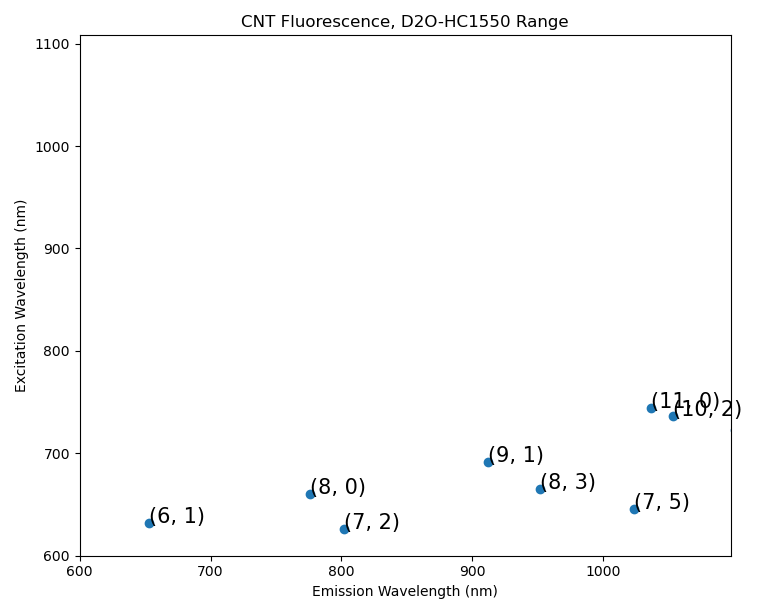
\includegraphics[width=9cm,height=7cm]{./Figures/CNTs/HC1550_range.png}
		\caption{ 1550HC CNTs }
		\label{fig:cnt1550}
	\end{minipage}
\end{figure}
\clearpage
